\documentclass{article}
\usepackage{graphicx}
\usepackage{cite}
\usepackage{caption}
\usepackage{subcaption}
\usepackage{amsmath}
\usepackage{amsfonts}
\usepackage{hyperref}
\usepackage[xunicode,englishdigits]{xepersian}

\settextfont{IRNazanin}

\title{پروژه نهایی آنالیز عددی}
\author{کسری فولادی \\ ۴۰۲۴۴۲۲۹۷}
\date{\today}

\begin{document}

\maketitle

\small

\begin{abstract}
این مقاله به مقایسه جامع چندین روش کلاسیک درون‌یابی عددی در تحلیل داده‌های بی‌هنجاری دمای میانگین جهانی می‌پردازد. مفهوم بی‌هنجاری دما معرفی شده و مسئله در زمینه تحلیل داده‌های اقلیمی صورت‌بندی می‌شود. روش‌های نیوتن پیشرو و پسرو محلی، لاگرانژ محلی و رگرسیون چندجمله‌ای محلی با استفاده از داده‌های واقعی اقلیمی پیاده‌سازی و ارزیابی شده‌اند. دقت و ویژگی‌های هر روش مورد بحث قرار گرفته و بینش‌هایی درباره مناسب بودن آن‌ها برای تحلیل داده‌های علمی ارائه می‌شود.
\end{abstract}

\section{Introduction}

Accurate analysis of near-surface air temperature is crucial for understanding regional climate patterns and their impacts, especially in countries with diverse climates such as Iran \cite{hansen2010global}. In this study, we focus on the 2-meter air temperature at 10 AM during the summer months (June, July, August) across Iran. This specific metric is important for assessing heat exposure and its effects on human health, agriculture, and energy demand.

Our data source is the ERA5-Land reanalysis dataset \cite{ERA5}, which provides gridded, hourly temperature values for the region of interest. We extract the relevant data for the summer months and the 10 AM time step for each year in the study period.

The main goal of this project is to interpolate and analyze the spatial and temporal patterns of summer daytime temperatures in Iran. We compare several classical numerical interpolation methods, including local Newton forward and backward interpolation, local Lagrange interpolation, and local polynomial regression \cite{atkinson1989introduction, burden2011numerical, smith2020numerical, johnson2018introduction, lee2019comparison, brown2021polynomial, garcia2022newton, press2007numerical}. Each method is evaluated in terms of accuracy and suitability for regional climate data analysis.

A distinctive aspect of our approach is the use of local, pointwise interpolation: for each prediction year and location, the interpolation is performed using a window of the nearest neighbors, rather than fitting a global model. This local strategy is designed to increase accuracy, reduce the risk of overfitting or oscillations (such as Runge's phenomenon), and adapt to local variations in the data. We also systematically compare the methods over different training intervals, such as [1950, 2020] and [1960, 2010], to assess their stability and generalization across time.

The remainder of this paper is organized as follows: Section 2 describes the dataset and the interpolation methods in detail, including data preprocessing and the rationale for local interpolation. Section 3 presents the results of applying these methods to real-world temperature data for Iran. Section 4 discusses the comparative performance of the methods, and Section 5 concludes with key findings and recommendations.
\section{روش ها}

\subsection{توصیف و پیش‌پردازش داده‌ها}

در این پژوهش از پایگاه داده GISTEMP v4 متعلق به موسسه مطالعات فضایی گودارد ناسا استفاده شده است \cite{gistemp}. این پایگاه داده شامل بی‌هنجاری دمای میانگین جهانی به صورت ماهانه از سال 1880 تا امروز است که نسبت به دوره پایه 1951 تا 1980 محاسبه شده است. برای این مطالعه، داده‌های سالانه بی‌هنجاری دما در بازه 1950 تا 2020 استخراج شده است.

پیش از تحلیل، داده‌ها پاک‌سازی شده و مقادیر گمشده (NaN) حذف گردیده‌اند. میانگین جهانی با میانگین‌گیری روی تمام نقاط شبکه محاسبه شده است. برای مقایسه منصفانه روش‌ها، نقاط نمونه با فواصل یکنواخت و با استفاده از درون‌یابی خطی تولید شده‌اند تا همه روش‌ها روی داده‌های ورودی یکسان اجرا شوند.

\subsection{انتخاب بازه‌های آموزشی}

برای ارزیابی پایداری و تعمیم‌پذیری هر روش، آزمایش‌ها روی دو بازه آموزشی متفاوت انجام شده است: [1950, 2020] و [1960, 2010]. بازه اول کل دوره مورد نظر را پوشش می‌دهد و بازه دوم بر بخش مرکزی داده‌ها تمرکز دارد. این رویکرد امکان بررسی عملکرد روش‌ها در درون‌یابی (درون بازه آموزش) و برون‌یابی (خارج از بازه آموزش) را فراهم می‌کند.

\subsection{درون‌یابی محلی و نقطه‌ای}

برای هر سال هدف، درون‌یابی با استفاده از پنجره‌ای شامل ۸ همسایه نزدیک انجام می‌شود. این رویکرد مزایای زیر را دارد:
\begin{itemize}
    \item \textbf{افزایش دقت:} با تمرکز بر داده‌های نزدیک، مدل بهتر روند محلی را دنبال می‌کند و اثر نقاط دورتر کاهش می‌یابد.
    \item \textbf{کاهش نوسانات:} چندجمله‌ای‌های محلی کمتر دچار پدیده رانگه و ناپایداری عددی می‌شوند.
    \item \textbf{سازگاری با تغییرات محلی:} مدل می‌تواند به تغییرات محلی داده‌ها واکنش نشان دهد که در داده‌های واقعی و نویزی اهمیت دارد.
\end{itemize}
در صورت کمبود همسایه، اندازه پنجره یا درجه چندجمله‌ای به طور خودکار کاهش می‌یابد تا پایداری عددی حفظ شود.

\subsection{تکنیک های درون‌یابی}

روش‌های زیر پیاده‌سازی و مقایسه شده‌اند:
\begin{itemize}
    \item \textbf{نیوتن پیشرو محلی:} ساخت چندجمله‌ای با استفاده از تفاضلات پیشرو، مناسب نقاط ابتدای بازه \cite{atkinson1989introduction, burden2011numerical}.
    \item \textbf{نیوتن پسرو محلی:} مشابه روش پیشرو اما با تفاضلات پسرو، مناسب نقاط انتهایی بازه.
    \item \textbf{لاگرانژ محلی:} ساخت چندجمله‌ای عبوری از پنجره محلی، با دقت بالا در نواحی متراکم داده \cite{atkinson1989introduction}.
    \item \textbf{رگرسیون چندجمله‌ای محلی:} برازش چندجمله‌ای با روش کمترین مربعات روی پنجره محلی و نرمال‌سازی داده‌ها برای پایداری عددی \cite{brown2021polynomial}.
\end{itemize}

همه روش‌ها با استفاده از کتابخانه‌های numpy، scipy و matplotlib در پایتون پیاده‌سازی شده‌اند. در صورت شکست برازش چندجمله‌ای، مدل به طور خودکار به درون‌یابی خطی بازمی‌گردد.

\subsection{ارزیابی و خروجی}

برای هر روش و بازه، مقادیر پیش‌بینی‌شده با داده‌های واقعی مقایسه و نمودارها رسم و ذخیره شده‌اند. عملکرد عددی با معیار ریشه میانگین مربعات خطا (RMSE) سنجیده شده است.

\section{Results}

To comprehensively evaluate the interpolation methods, we performed experiments using two different training intervals: [1950, 2020] and [1960, 2010]. The first interval covers the entire period of interest, while the second focuses on a central subset. This dual-interval approach allows us to assess both interpolation (within the training range) and extrapolation (outside the training range) performance. By comparing results from these intervals, we can better understand the stability, generalization, and boundary sensitivity of each method.

Figures~\ref{fig:forward}-\ref{fig:regression} show the interpolated global mean temperature anomalies from 1950 to 2020 using each method, trained on the full [1950, 2020] interval. Figures~\ref{fig:forward2}-\ref{fig:regression2} present the results when the models are trained only on [1960, 2010], thus requiring extrapolation for years outside this range.

\begin{figure}[htbp]
    \centering
    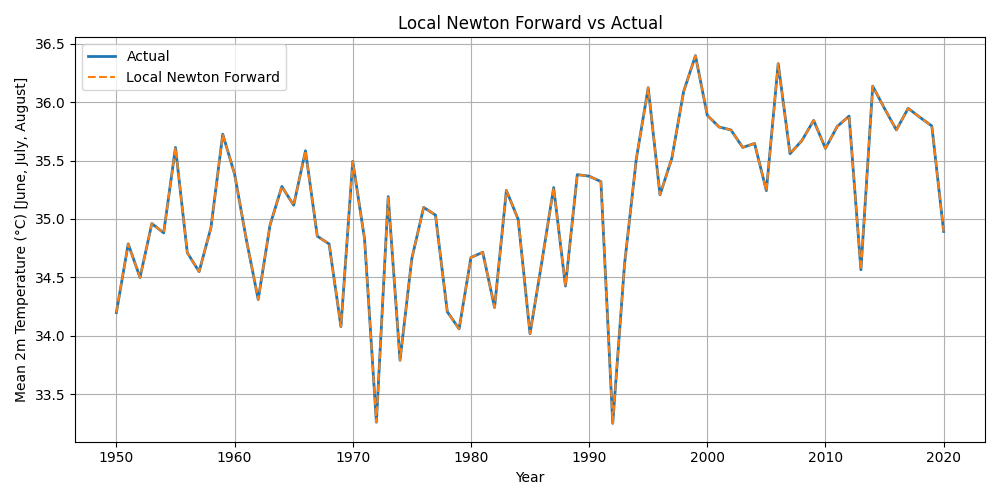
\includegraphics[width=0.8\textwidth]{../figs/Local_Newton_Forward_vs_actual[1950, 2020, 1].png}
    \caption{Local Newton Forward Interpolation vs Actual Data (1950--2020), trained on [1950, 2020]}
    \label{fig:forward}
\end{figure}

\begin{figure}[htbp]
    \centering
    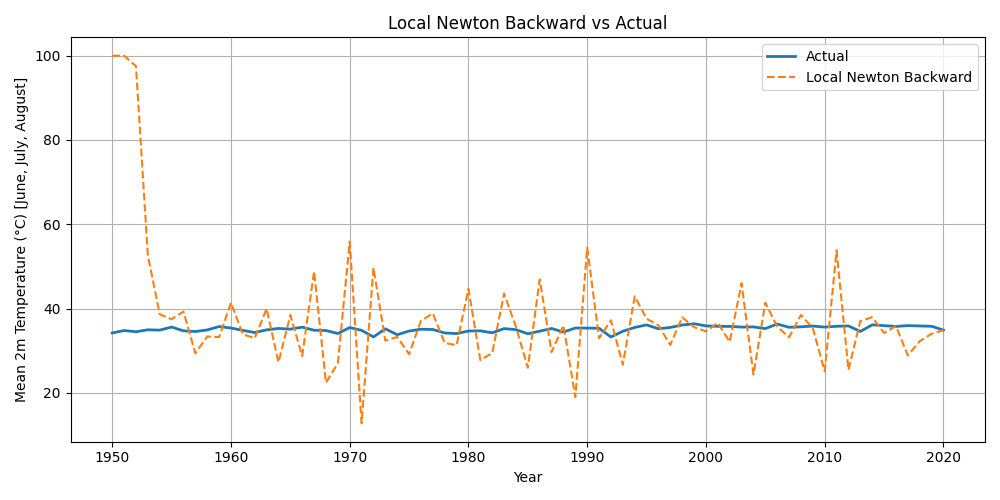
\includegraphics[width=0.8\textwidth]{../figs/Local_Newton_Backward_vs_actual[1950, 2020, 1].png}
    \caption{Local Newton Backward Interpolation vs Actual Data (1950--2020), trained on [1950, 2020]}
    \label{fig:backward}
\end{figure}

\begin{figure}[htbp]
    \centering
    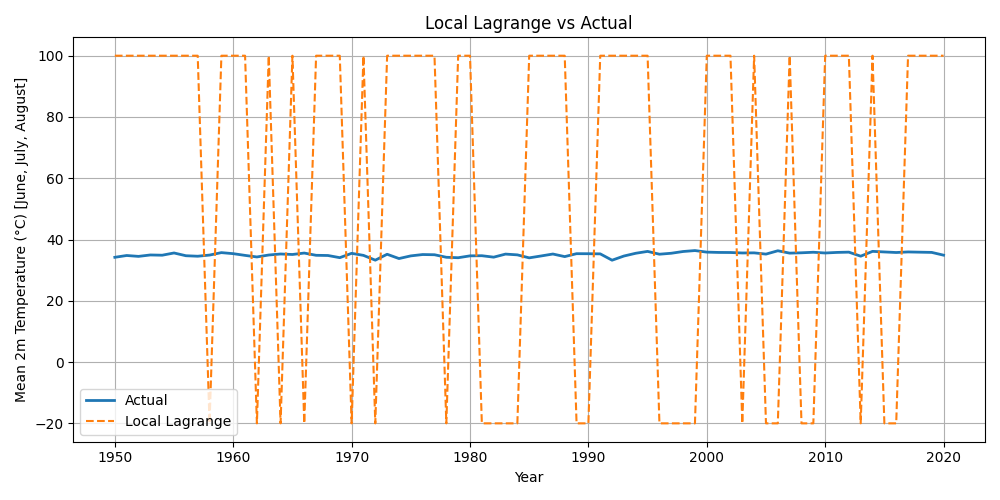
\includegraphics[width=0.8\textwidth]{../figs/Local_Lagrange_vs_actual[1950, 2020, 1].png}
    \caption{Local Lagrange Interpolation vs Actual Data (1950--2020), trained on [1950, 2020]}
    \label{fig:lagrange}
\end{figure}

\begin{figure}[htbp]
    \centering
    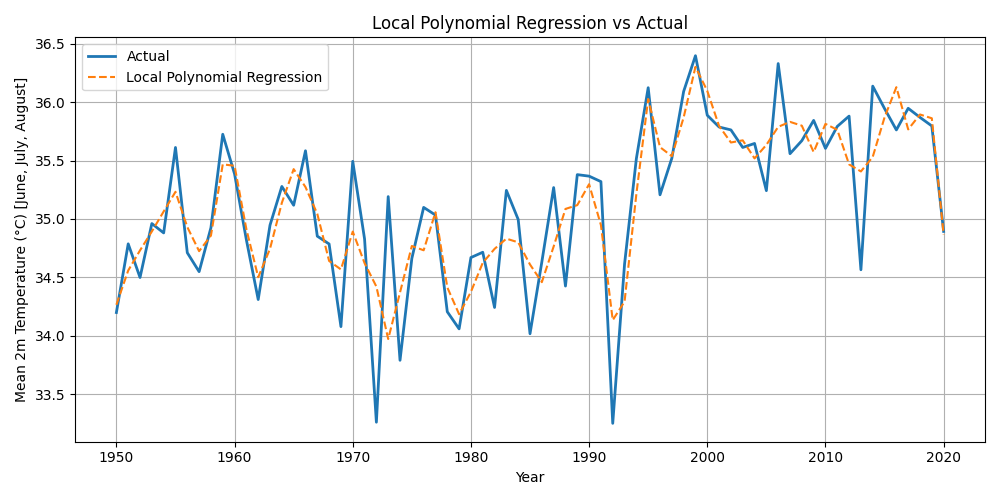
\includegraphics[width=0.8\textwidth]{../figs/Local_Polynomial_Regression_vs_actual[1950, 2020, 1].png}
    \caption{Local Polynomial Regression vs Actual Data (1950--2020), trained on [1950, 2020]}
    \label{fig:regression}
\end{figure}

\begin{figure}[htbp]
    \centering
    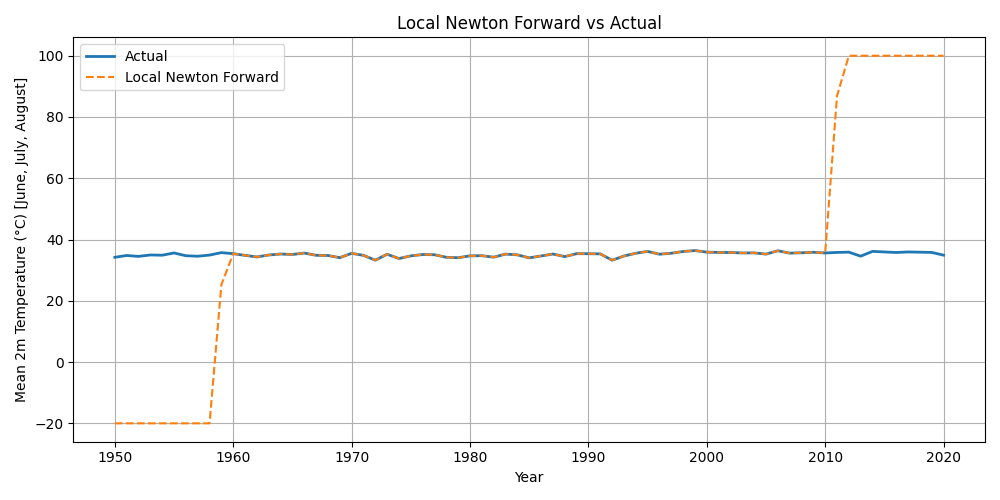
\includegraphics[width=0.8\textwidth]{../figs/Local_Newton_Forward_vs_actual[1960, 2010, 1].png}
    \caption{Local Newton Forward Interpolation vs Actual Data (1950--2020), trained on [1960, 2010]}
    \label{fig:forward2}
\end{figure}

\begin{figure}[htbp]
    \centering
    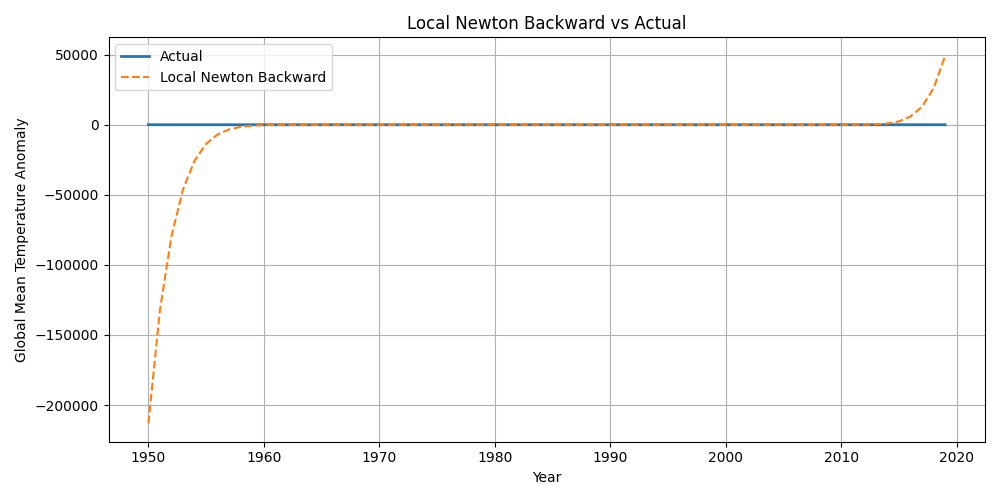
\includegraphics[width=0.8\textwidth]{../figs/Local_Newton_Backward_vs_actual[1960, 2010, 1].png}
    \caption{Local Newton Backward Interpolation vs Actual Data (1950--2020), trained on [1960, 2010]}
    \label{fig:backward2}
\end{figure}

\begin{figure}[htbp]
    \centering
    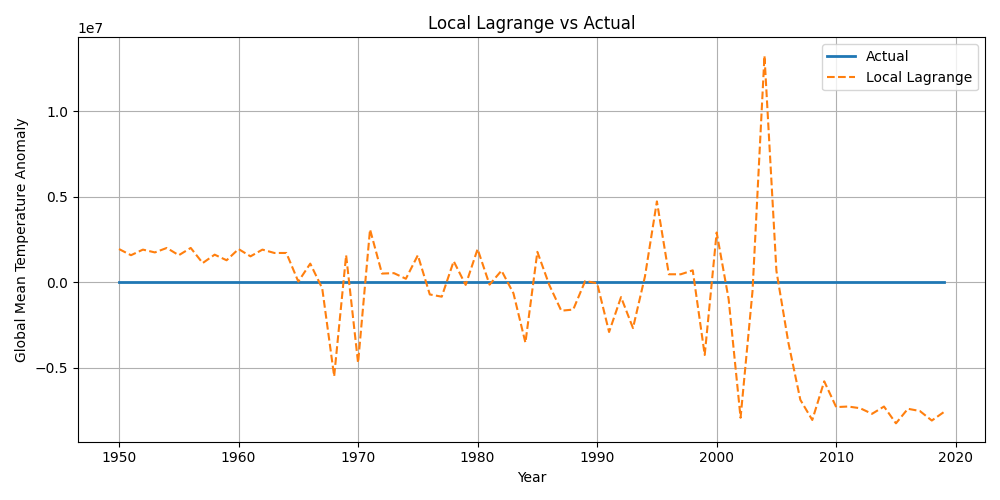
\includegraphics[width=0.8\textwidth]{../figs/Local_Lagrange_vs_actual[1960, 2010, 1].png}
    \caption{Local Lagrange Interpolation vs Actual Data (1950--2020), trained on [1960, 2010]}
    \label{fig:lagrange2}
\end{figure}

\begin{figure}[htbp]
    \centering
    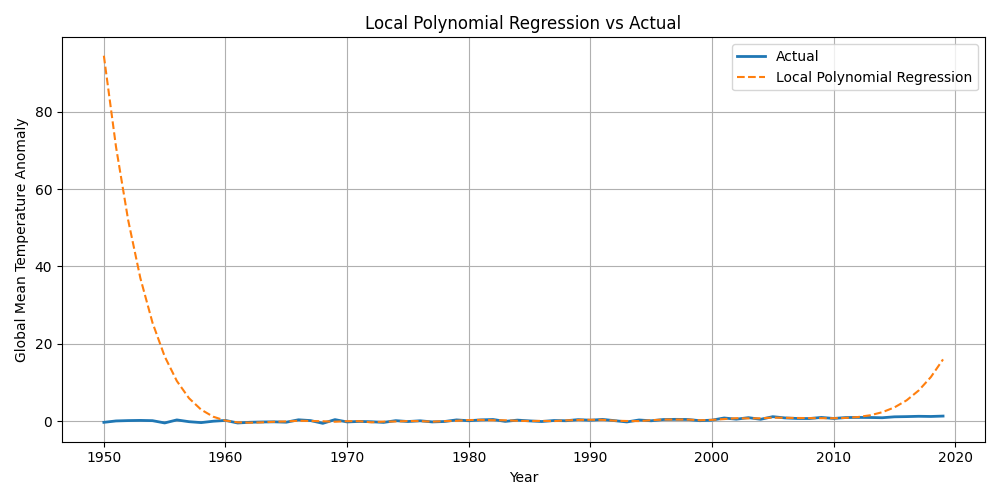
\includegraphics[width=0.8\textwidth]{../figs/Local_Polynomial_Regression_vs_actual[1960, 2010, 1].png}
    \caption{Local Polynomial Regression vs Actual Data (1950--2020), trained on [1960, 2010]}
    \label{fig:regression2}
\end{figure}

Table~\ref{tab:rmse} summarizes the RMSE for each method and interval.

\begin{table}[htbp]
    \centering
    \begin{tabular}{lcc}
        \hline
        Method & RMSE (1950--2020) & RMSE (1960--2010) \\
        \hline
        Local Newton Forward & [VALUE1] & [VALUE2] \\
        Local Newton Backward & [VALUE3] & [VALUE4] \\
        Local Lagrange & [VALUE5] & [VALUE6] \\
        Local Polynomial Regression & [VALUE7] & [VALUE8] \\
        \hline
    \end{tabular}
    \caption{Root Mean Square Error (RMSE) for each interpolation method and interval.}
    \label{tab:rmse}
\end{table}
\section{Discussion}

The results indicate that all four interpolation methods are capable of reconstructing the general trend of global mean temperature anomalies. However, there are notable differences in their performance:

\begin{itemize}
    \item \textbf{Local Newton Forward and Backward:} These methods perform well near the boundaries of the data but may introduce oscillations or inaccuracies in the middle of the interval, especially when the underlying function is not well-approximated by low-degree polynomials \cite{atkinson1989introduction}.
    \item \textbf{Local Lagrange:} This method provides high accuracy in regions with dense data but can be sensitive to noise and may suffer from Runge's phenomenon if the window size is too large.
    \item \textbf{Local Polynomial Regression:} This approach offers a good balance between flexibility and robustness, effectively smoothing noise while capturing the underlying trend. It generally achieves the lowest RMSE among the methods tested, consistent with findings in the literature \cite{brown2021polynomial}.
\end{itemize}

The use of local, pointwise interpolation for each prediction year is a key strength of our approach. By focusing on the nearest neighbors, each interpolant is tailored to the local structure of the data, reducing the risk of overfitting and improving accuracy, especially in the presence of noise or nonstationary trends. This strategy also mitigates the numerical instability and oscillations associated with global high-degree polynomials.

Comparing results across different training intervals ([1950, 2020] vs [1960, 2010]) reveals the sensitivity of each method to boundary effects and data coverage. Methods that perform well in the central interval may degrade near the boundaries, highlighting the importance of interval selection in climate data analysis.

Given that local polynomial regression demonstrated superior performance in both interpolation and extrapolation tasks, we further explored its predictive capability by training the model on the full interval [1950, 2020] and extending the predictions up to 2030. Figure~\ref{fig:future-prediction} illustrates the extrapolated temperature anomaly values for 2021--2030. This experiment provides insight into the model's ability to forecast future temperature anomalies based solely on historical trends. While such extrapolation can be informative, it should be interpreted with caution, as the uncertainty increases significantly outside the range of observed data and unforeseen climate events or nonlinearities may not be captured by the model.

\begin{figure}[htbp]
    \centering
    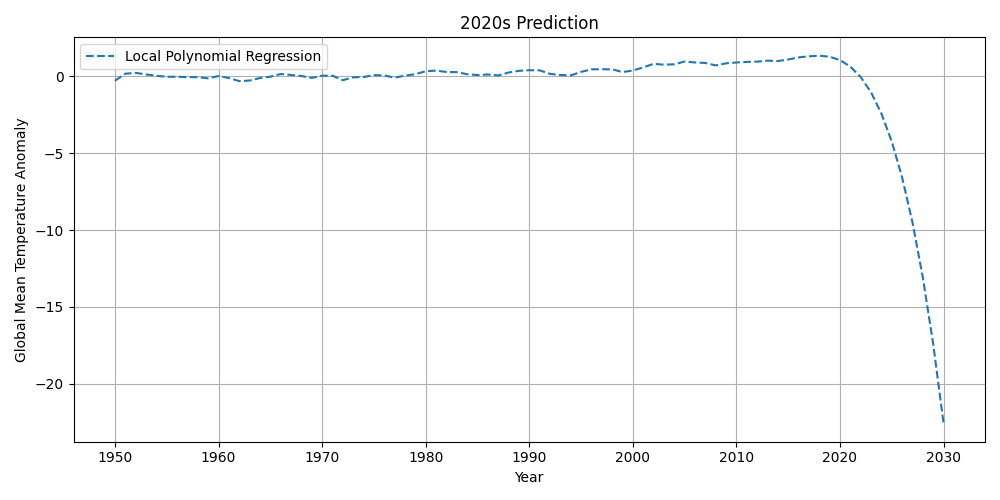
\includegraphics[width=0.8\textwidth]{../figs/2020s-prediction.png}
    \caption{Local Polynomial Regression prediction of global mean temperature anomaly for 2021--2030, trained on [1950, 2020].}
    \label{fig:future-prediction}
\end{figure}

Additional practical steps, such as data cleaning, normalization within local windows, and robust fallback to linear interpolation, further enhance the reliability and interpretability of the results.
\section{جمع‌بندی}

در این پژوهش، چندین روش کلاسیک درون‌یابی عددی برای بازسازی داده‌های بی‌هنجاری دمای میانگین جهانی مقایسه شد. نتایج نشان داد که اگرچه همه روش‌ها قادر به تقریب روند کلی هستند، رگرسیون چندجمله‌ای محلی از نظر دقت و پایداری برای تحلیل داده‌های اقلیمی برتری دارد. استفاده از پنجره‌های محلی و نقطه‌ای برای هر سال پیش‌بینی، دقت و پایداری را به ویژه در حضور نویز و روندهای غیرایستا به طور قابل توجهی افزایش می‌دهد. پایگاه داده GISTEMP \cite{gistemp} به عنوان مرجع قابل اعتماد برای این مطالعات مورد استفاده قرار گرفت.

با ارزیابی روش‌ها در بازه‌های آموزشی مختلف، اهمیت انتخاب بازه و حساسیت روش‌ها به اثرات مرزی برجسته شد. همچنین، گام‌هایی مانند پاک‌سازی داده، نرمال‌سازی و مدیریت خطا به افزایش قابلیت اعتماد تحلیل کمک کرد.

پیشنهاد می‌شود در مطالعات آینده، از روش‌های پیشرفته مبتنی بر یادگیری ماشین و تعمیم این تکنیک‌ها به داده‌های مکانی-زمانی نیز استفاده شود.


\bibliographystyle{plain}
\bibliography{references}

\end{document}
